%
% CMPT 454: Database Systems II - A Course Overview
% Section: Indexed File Structure
%
% Author: Jeffrey Leung
%

\section{Indexed File Structure}
	\label{sec:indexing}

\subsection{Introduction}
	\label{subsec:indexing-introduction}
\begin{easylist}

& \textbf{Indexed file structure:} File organization structure where records are organized and searchable by certain configured search keys
	&& Designed to be efficient for value-based searches

& Structure of an index:

	&& \textbf{Search key:} Field(s) on which a file/record is organized for searchability
		&&& Not guaranteed to be unique
		&&& Creating an index associates each record with a corresponding search key
		&&& \textbf{Composite search key:} Search key composed of multiple fields
			&&&& Sorting by a composite key sorts by its fields in order

	&& \textbf{Data entry:} Single search key and IDs of all records which contain/match it
		&&& Notation: Given search key value $k$, the index emits a set of data entries $k*$
		&&& Always sorted by the search key $k$
		&&& Possible formats:
			&&&& $\langle k \textrm{, data record} \rangle$
				&&&&& DB cannot have any other indices
			&&&& $\langle k \textrm{, RID} \rangle$
			&&&& $\langle k \textrm{, list of RIDs} \rangle$

\end{easylist}
\subsection{Types of Indices}
	\label{subsec:types-of-indices}
\begin{easylist}
		
& Methods of indexing:
	&& \textbf{Sorted file structure:} Indexed file structure where records are sorted by search key (generally using a tree)
		&&& Efficient for equality/range searches
		
	&& \textbf{Hashed file structure:} Indexed file structure where records are grouped in buckets by a hashed search key
		&&& Efficient for equality searches
		&&& Types: Static hashing, extendible hashing, linear hashing

& \textbf{Unique index:} Index format where the search key contains a candidate key
	&& \textbf{(Candidate) Key:} Set of fields which uniquely defines a record
	&& I.e. Searching the index using a candidate key returns either 0 or 1 result

& \textbf{Clustered index:} Index for which the data records are sorted by $k$ (in addition to the data entries sorted by $k$)
	&& Maximum of 1 clustered index per file
	&& Records are sequential on the page, though the pages may have pointers to the next page rather than be sequential
	&& Diagram: See figure~\ref{img:clustered-index}

	\begin{figure}[!htb]
		\centering
		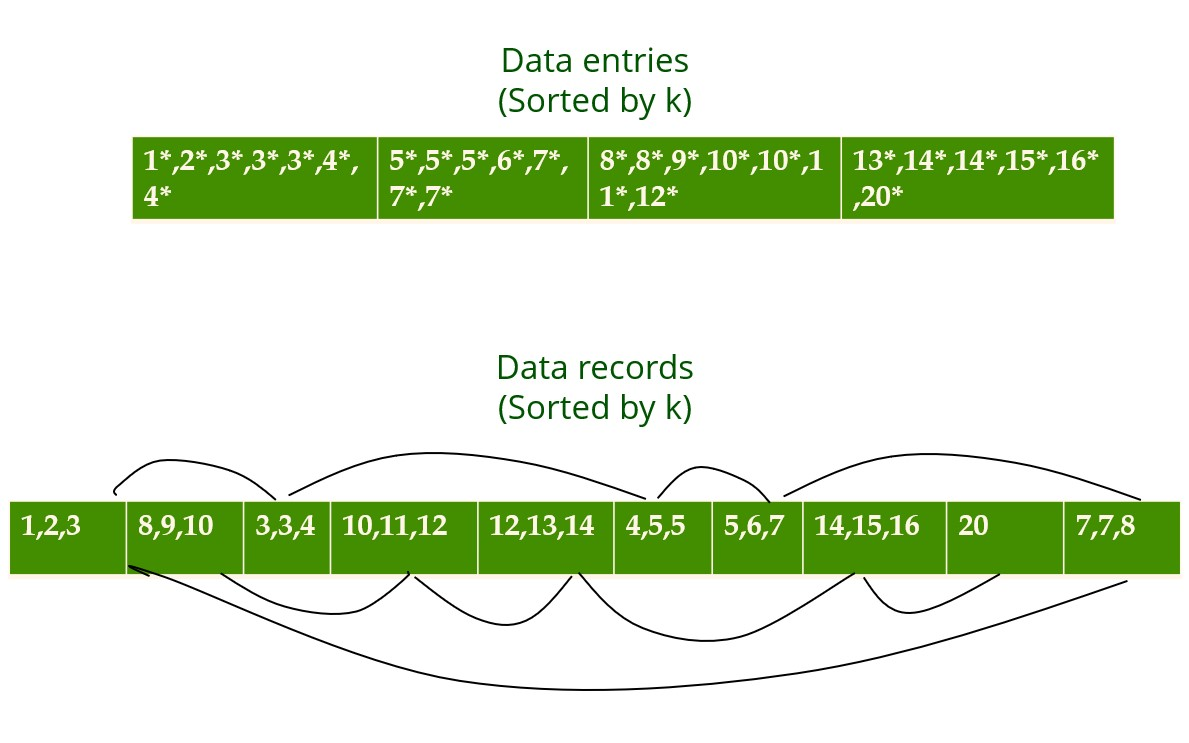
\includegraphics[width=.8\linewidth]{indexed-file-structure/clustered-index}
		\caption{A clustered index and its records}
		\label{img:clustered-index}
	\end{figure}
	
	&& \textit{Unclustered index:} Index for which the data records are not sorted by $k$
		&&& Diagram: See figure~\ref{img:unclustered-index}

		\begin{figure}[!htb]
			\centering
			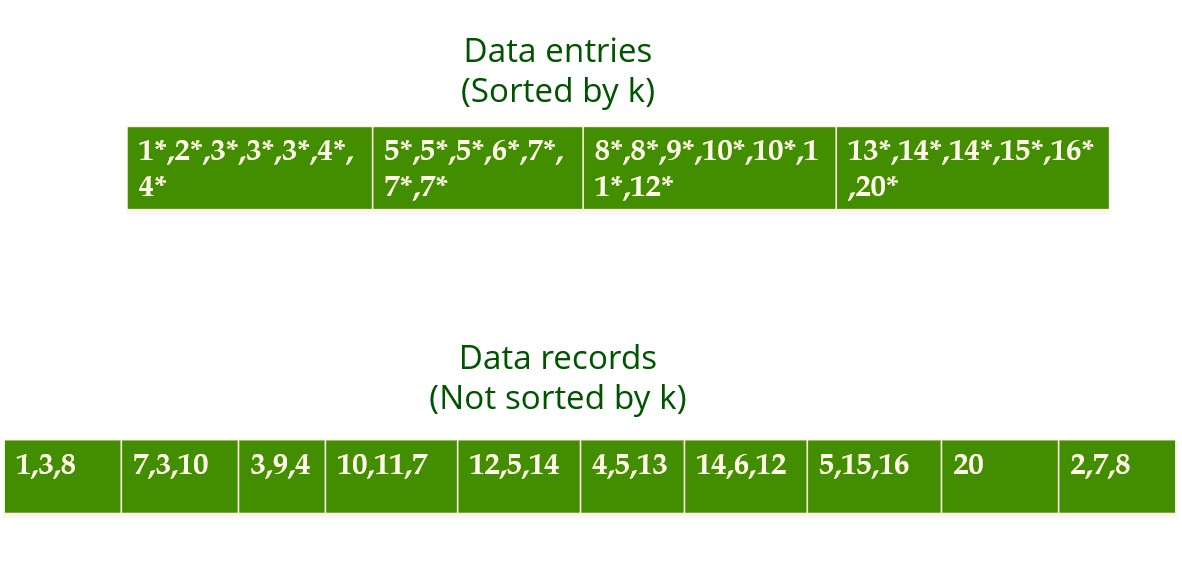
\includegraphics[width=.8\linewidth]{indexed-file-structure/unclustered-index}
			\caption{An un clustered index and its records}
			\label{img:unclustered-index}
		\end{figure}
	
	&& Data entry format $\langle k \textrm{, data record} \rangle$ is always clustered by the single index
	&& Search process for a given data range in a clustered index:
		&&& Use the data entry to find the page with the first value to read
		&&& Read through all data records in order until reaching a value greater than the end

& \textbf{Dense index:} Index where, for every search key $k$, there are one or more data entries $k*$
	&& Data entry format $\langle k \textrm{, data record} \rangle$ is always dense
	&& \textbf{Sparse index:} Index where there is at least one search key $k$ which does not map to any data entries
		&&& In a sparse index, data entries are always clustered for efficient scanning

\clearpage
\end{easylist}
\subsection{Tree-Structured Indexes}
	\label{subsec:tree-structured-indexes}
\begin{easylist}

& \textbf{Index search tree:} Search structure where index pages branch out to primary leaf pages which contain data entries
	&& Root and index pages consist of splitting keys and ordered pointers to trees containing values greater/less than the splitting keys
	&& Common components:
		&&& \textbf{Index pages:} Index search tree node which contains pivots for the search key values and pointers to index/leaf pages
			&&&& Does not directly contain data entries
			&&&& \textbf{Splitting key:} Index page value which acts as a pivot value for partitioned subtrees
			&&&& Root: Top node of an index search tree which contains a single pivot value and pointers to index pages
		&&& \textbf{Primary leaf page:} Index search tree leaf node which contains a set of data entries with pointers to data records
			&&&& Will not be deallocated even if empty

\clearpage
\end{easylist}
\subsubsection{ISAM Trees}
	\label{subsubsec:isam-trees}
\begin{easylist}

& \textbf{Indexed sequential access method (ISAM):} Index search tree where index pages are static and leaf pages contain optional overflow pages
	&& \textbf{Overflow page:} Linked list starting from a primary leaf page, which contains additional search key values
		&&& Allocated/deallocated as required; all other nodes in the tree are not affected during insert/delete operations
		&&& Can degrade performance

& Diagram: See figure~\ref{img:isam-tree}
	
\begin{figure}[!htb]
	\centering
	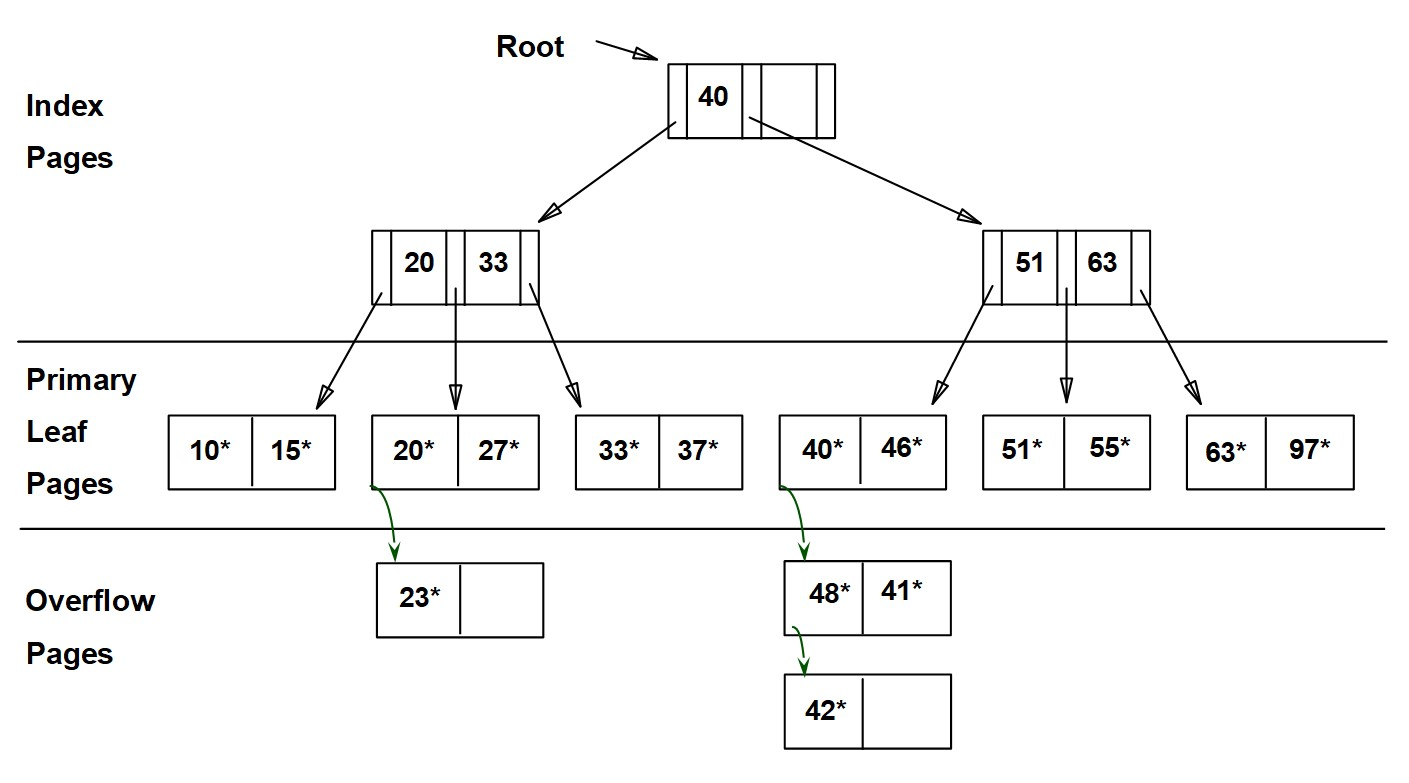
\includegraphics[width=.8\linewidth]{indexed-file-structure/isam-tree}
	\caption{An ISAM Tree}
	\label{img:isam-tree}
\end{figure}

& Search process:
	&& Follow the search from the root through the index pages to the matching primary leaf page
	&& Search the leaf page
	&& Search any linked overflow pages until a result is found
& Rebalanced during system maintenance

\clearpage
\end{easylist}
\subsubsection{B+ Trees}
	\label{subsubsec:b+-trees}
\begin{easylist}

& \textbf{B+ tree:} Index search tree which dynamically rebalances nodes and children during operation

& Diagram: See figure~\ref{img:bplus-tree}
	
\begin{figure}[!htb]
	\centering
	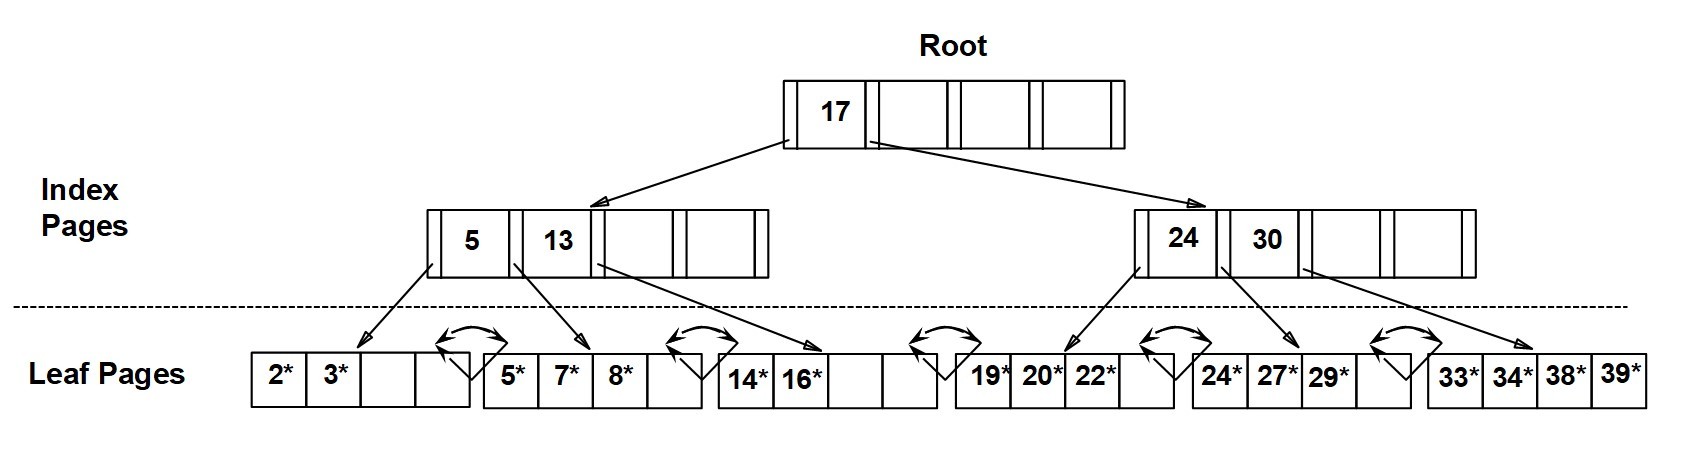
\includegraphics[width=.8\linewidth]{indexed-file-structure/bplus-tree}
	\caption{A B+ Tree}
	\label{img:bplus-tree}
\end{figure}
	
& \textbf{Order:} Minimum and maximum splitting key capacity of a B+ tree (which can differ for index and leaf nodes)
	&& Denoted by $d$
	&& Each B+ tree node must have between $d$ and $2d$ search keys (inclusive), except for the root (minimum 1)
	&& \textit{Fanout:} Branching factor of a B+ tree
		&&& Denoted by $F$
		&&& Fanout of root: $2$ to $2d+1$
		&&& Fanout of index nodes: $d+1$ to $2d+1$
		&&& Fanout of leaf nodes: $d$ to $2d$

& Ensures insert/delete/search operations are $\log_{F} N$ where $N = $ number of leaf nodes
	
& Operations:
	&& \textbf{Copying up:} B+ tree operation where a search key in a leaf is copied to the parent index node
		&&& Used when splitting a leaf in two
					
	&& \textbf{Pushing up:} B+ tree operation where a splitting key in an index node is moved to the parent index node, and removed from the original
		&&& Used when splitting an index node in two
		
	&& Insertion into a full leaf node:
		&&& Split leaf $L$ into two nodes, $L$ and $L2$
		&&& Redistribute entries evenly
		&&& Copy up the middle key to the parent to create a new partition
		&&& Link $L2$ to the parent
		&&& If the parent index node is not being split, the process is repeated recursively but with pushing-up instead of copying-up
			
	&& Deletion:
		&&& Search for and remove the entry
		&&& If the leaf node which contained the entry has only $d-1$ entries remaining:
			&&&& If the sibling node has more than $d-1$ entries, then re-balance entries with the sibling so both have at least $d-1$ entries
			&&&& Else, merge the node and its sibling (with $d$ entries) to create a node of $2d-1$ entries
				&&&&& Delete the key pointing to the deleted leaf node
				&&&&& Propagate merge upwards recursively
		
	&& \textbf{Bulk loading:} Initialization of a B+ tree with a number of records, which avoids constant rebalancing through standard insertion
		&&& Process:
			&&&& Sort data entries by search key
			&&&& Allocate data entries on the disk
			&&&& Create parent nodes for data entry leaf pages from left to right
			&&&& If the parent of the current index node has more slots available, split index nodes into siblings
			&&&& If the parent of the current index node has no slots available, split the parent node

\clearpage
\end{easylist}
\subsection{Hash-Based Indices}
	\label{subsec:hash-based-indices}
\begin{easylist}

& \textbf{Hash-based index:} Search structure where primary pages, each identified by a hashed search key, point to data entry pages
	&& Optimized for equality search; does not support range search
	&& Vulnerable to skewed hash distributions

& Common components:
	&& Hash function: Function which hashes a search key to a value
		&&& Denoted by $h(k)$ for a given data entry with search key $k$
		&&& Bucket to store the entry is chosen from $N$ buckets by calculating $h(k) \textrm{ mod } N$
	&& \textbf{Primary (bucket) page:} Hash-based index page identified by a hashed search key and containing/linking to a bucket with data entries
		&&& Always allocated sequentially for speed of access
	&& \textbf{Directory:} Collection of primary pages
		&&& Not in all types of hash indices
	&& \textbf{Overflow page:} Hash index page containing data entries, linked to from a primary page
		&&& Not in all types of hash indices
		&&& Allocated and de-allocated as required

\clearpage
\end{easylist}
\subsubsection{Static Hashing}
	\label{subsubsec:static-hashing}
\begin{easylist}

& \textbf{Static hashing:} Hash-based index method where the primary pages are never modified or deallocated
	&& Uses overflow pages to hold additional data entries
		&&& May create overflow chains when there are too many records, or hashes skew towards several values
		
& Diagram: See figure~\ref{img:static-hashing}
\begin{figure}[!htb]
	\centering
	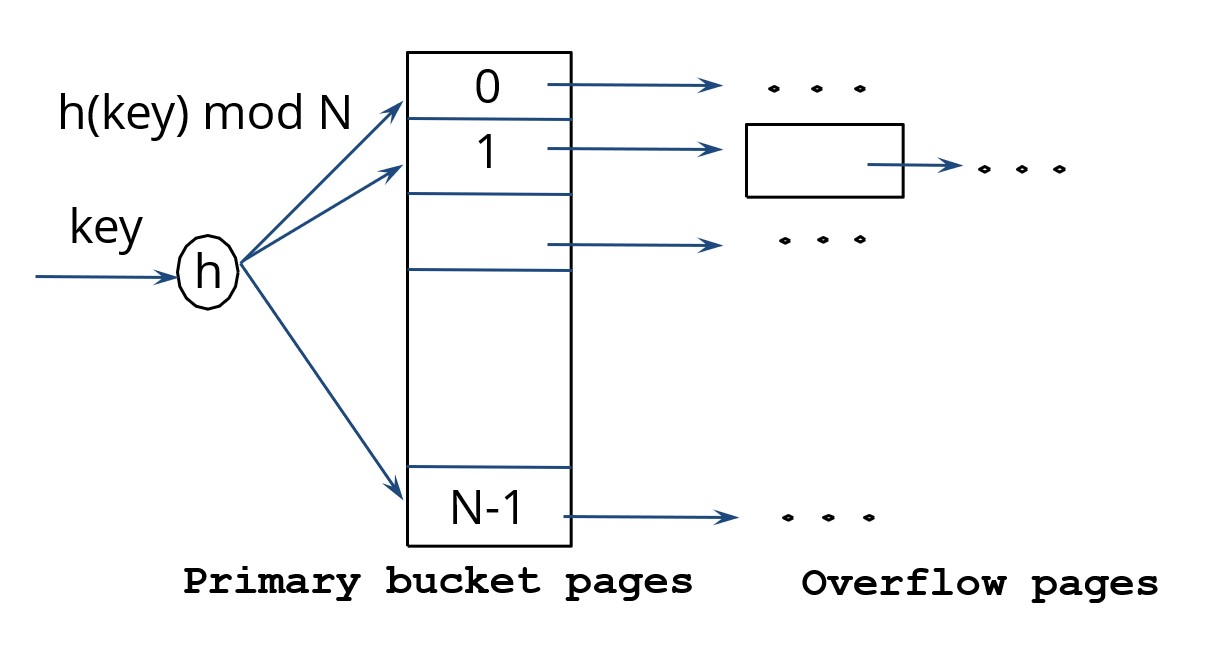
\includegraphics[width=.8\linewidth]{indexed-file-structure/static-hashing}
	\caption{A Static Hash Index}
	\label{img:static-hashing}
\end{figure}

\clearpage
\end{easylist}
\subsubsection{Extendible Hashing}
	\label{subsubsec:extendible-hashing}
\begin{easylist}

& \textbf{Extendible hashing:} Hash-based index method which splits overflowing buckets and dynamically increases the directory
	&& Does not use overflow pages
	&& When a bucket overflows, its contents are split into a new bucket which is added to the directory
	&& Requires accessing a directory page to look up an entry page
	&& Bucket access is approximately 1.2 page accesses amortized (due to overflows)

& \textbf{Global depth:} Value on an extendible hashing directory which tracks the number of bits in the current directory size
& \textbf{Local depth:} Value on an extendible hashing bucket which (approximately) tracks the number of buckets matching the same hash
	&& If local depth is less than global depth, then the bucket can be split without increasing directory size
	&& If local depth equals the global depth, then splitting the bucket will require doubling the directory
	
& Diagram: See figure~\ref{img:extendible-hashing}

\begin{figure}[!htb]
	\centering
	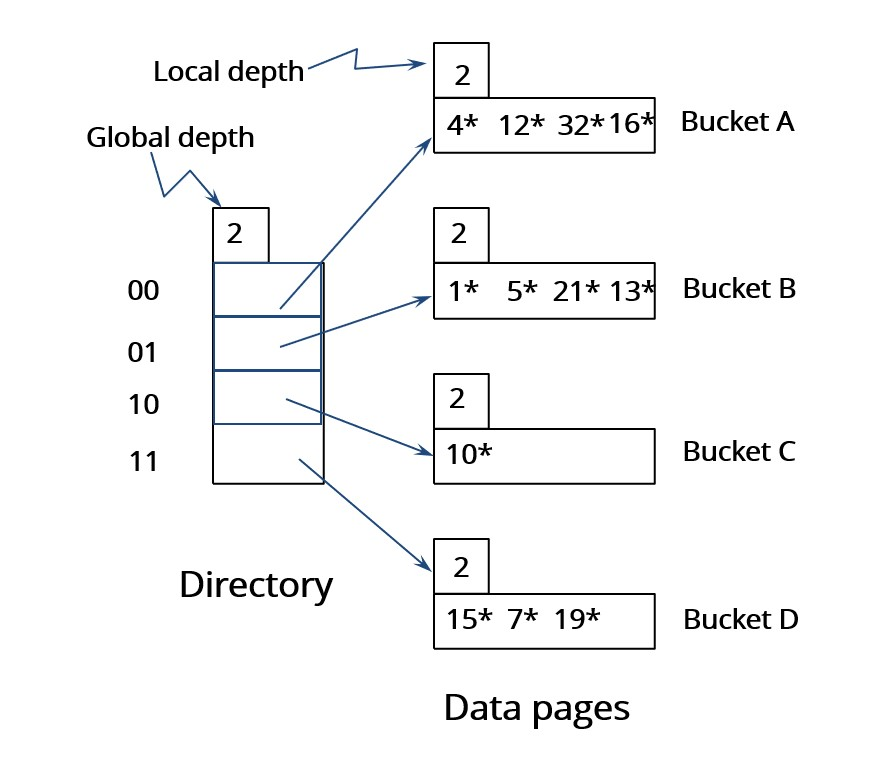
\includegraphics[width=.8\linewidth]{indexed-file-structure/extendible-hashing}
	\caption{An Extendible Hash Index}
	\label{img:extendible-hashing}
\end{figure}

\clearpage
& Operations:

	&& Insertion:
		&&& When a bucket overflows, split its contents into a new bucket of the same hash
		&&& Increment the local depth of both buckets
		&&& If the directory has no space for a new bucket of the same hash (i.e. the global depth is less than the new local depth), the directory is increased to accommodate hashing the new bucket:
			&&&& Double the directory (adding a new leftmost bit to the directory index)
			&&&& Increment the global depth
			&&&& Point the newly created directory indices to the existing buckets with the same hash values
		&&& Link the new duplicate hash value in the directory to the new bucket
		
		&&& Diagram: See figure~\ref{img:extendible-hashing-splitting}
		\begin{figure}[!htb]
			\centering
			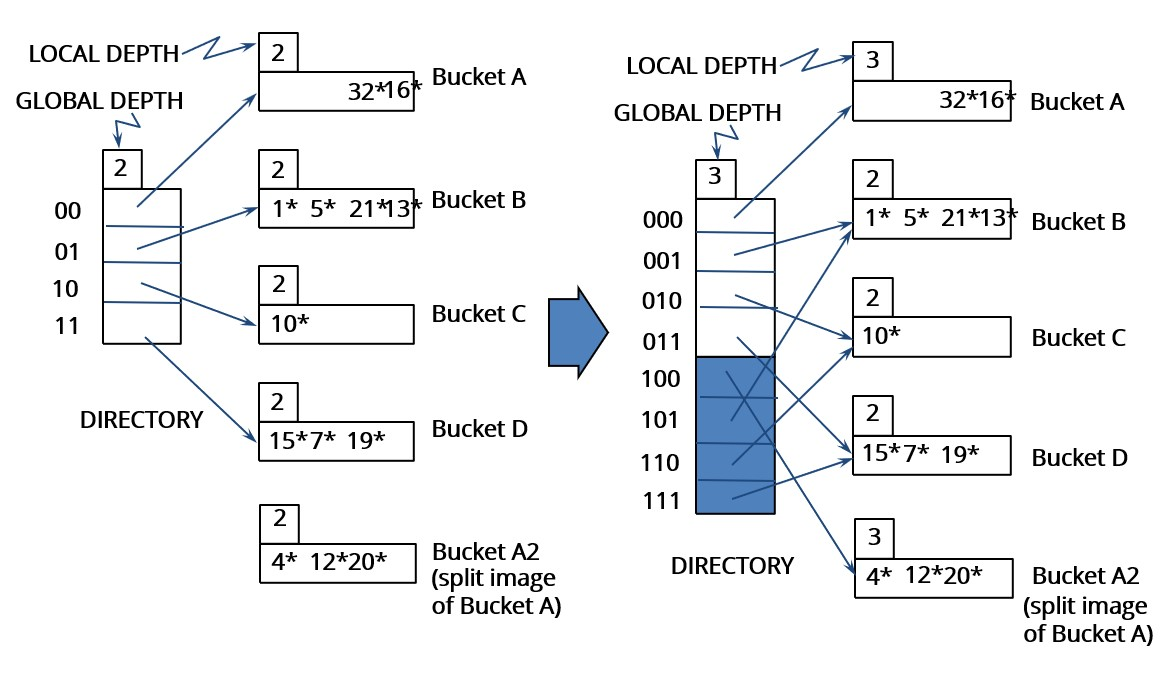
\includegraphics[width=.8\linewidth]{indexed-file-structure/extendible-hashing-splitting}
			\caption{Splitting an Extendible Hash Bucket}
			\label{img:extendible-hashing-splitting}
		\end{figure}
		
	&& Deletion:
		&&& Remove the data entry from the corresponding bucket
		&&& If the bucket has no more entries, deallocate it and point the key in the directory to the matching bucket
		&&& If half or more of the buckets of all hashes are empty/deallocated, the directory can be halved

\clearpage
\end{easylist}
\subsubsection{Linear Hashing}
	\label{subsubsec:linear-hashing}
\begin{easylist}

& \textbf{Linear hashing:} Hash-based index method which uses overflow pages, splits buckets using a round-robin strategy, and dynamically doubles the buckets
	&& Has no directory; does not require directory page lookup before accessing an entry page
	&& Splits a bucket into two (chosen by round-robin strategy) whenever any overflow page is created
		&&& Every bucket is kept split evenly, rather than focusing on splitting heavy-use buckets
	&& Bucket access is approximately 1.2 page accesses amortized (due to overflows)
	
& Components:

	&& \textbf{Overflow page (linear hashing):} Data bucket which holds additional data entries matching the index, which have not yet been split into new buckets
	
	&& Uses two hash algorithms at any given time; when the buckets are doubled, the old one is discarded and a new hash algorithm is added

	&& \textbf{Level:} Index of the hash algorithms currently being used, and the number of times the buckets have been doubled
		&&& Begins at 0; increments without limit
		&&& Hash algorithm of a certain level $x$ is denoted by $h_x$

	&& \textbf{Next:} Beginning index of buckets in a linear hashing index which have not yet been split
		&&& Begins at 0; increments when a bucket is split; reset to 0 after splitting all buckets once
		&&& All buckets before \textrm{next} have been split in the current round-robin implementation
			&&&& All buckets after or including \textrm{next} have not yet been split in the current round-robin implementation

		
& Diagram: See figure~\ref{img:linear-hashing}
\begin{figure}[!htb]
	\centering
	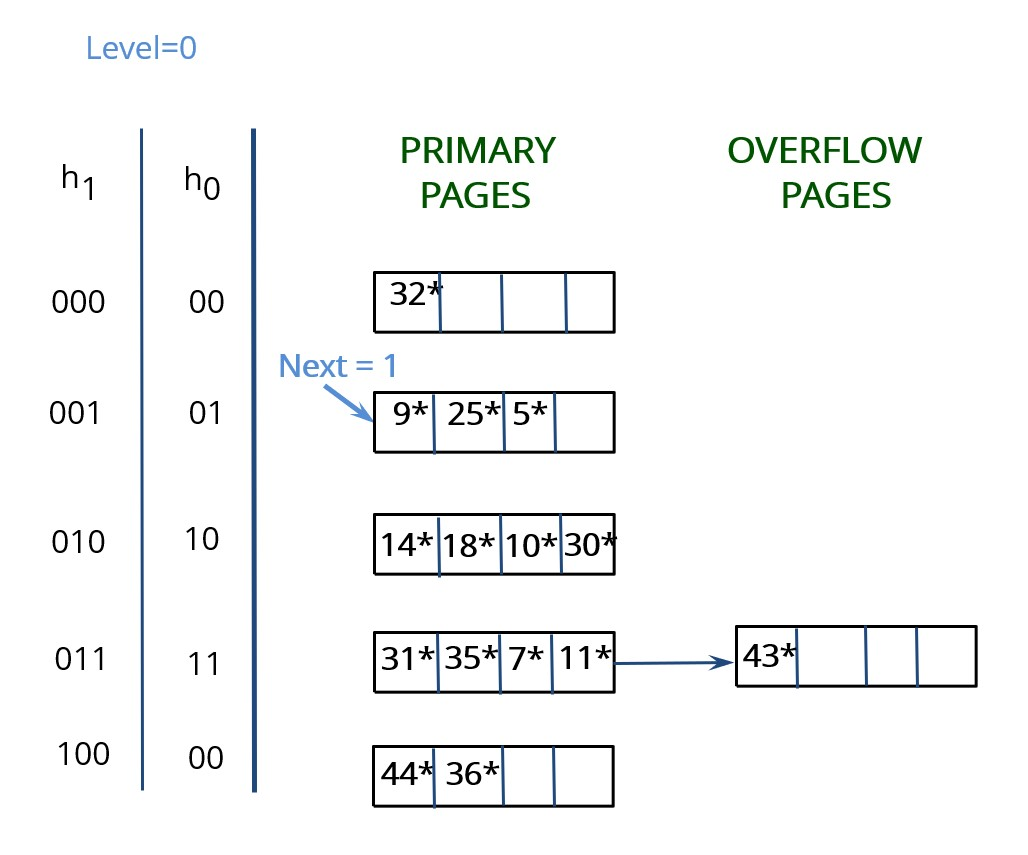
\includegraphics[width=.8\linewidth]{indexed-file-structure/linear-hashing}
	\caption{A Linear Hash Index}
	\label{img:linear-hashing}
\end{figure}
		
& Operations:	
			
	&& Search:
		&&& Use $h_\textrm{level}$ to find the index of the bucket where the value belongs
			&&&& If the index is less than \textrm{next}, the search key belongs in the index found by $h_\textrm{level+1}$ (as the bucket has been split)
			&&&& If the index is greater than or equal to \textrm{next}, the search key belongs in this (as the bucket has not yet been split)
		&&& Search the selected bucket and any linked overflow pages
	
	&& Insertion:
		&&& Apply the search process above to find the bucket to insert the data entry
		&&& Add the value to the bucket, creating an overflow page if necessary
		
		&&& If an overflow page is created:
			&&&& Split the bucket at index \textrm{next}
			&&&& Index the new bucket at the bottom of the others
			&&&& Use $h_\textrm{level+1}$ to redistribute the values between the old and new buckets
			&&&& Increment \textrm{next}
		
		&&& If \textrm{next} has looped through all buckets once (not including the newly split buckets):
			&&&& Discard hash algorithm $h_\textrm{level}$
			&&&& Increment \textrm{level}
			&&&& Create a new hash algorithm $h_\textrm{level+1}$
			&&&& Reset \textrm{next} to 0

\end{easylist}
\clearpage







































